\documentclass[english]{article}
\usepackage{notestemplate}
\usepackage{databases2}

\begin{document}

\makecover{Data bases 2}{2022/2023}

\section{Introduction}

\subsection{Architecture of the \dbms}

A \textbf{\dbms} \textit{(short for Data Base Management System)} is a system \textit{(or software product)} capable of managing data collections that can be:

\begin{itemize}
  \item \textbf{Large}
        \begin{itemize}[label=\(\rightarrow\)]
          \item much larger than the central memory available on the computer that runs the software
          \item often data must be stored on secondary storage devices
        \end{itemize}
  \item \textbf{Persistent}
        \begin{itemize}[label=\(\rightarrow\)]
          \item its lifespan is longer than the lifespan of the software that accesses it
        \end{itemize}
  \item \textbf{Shared}
        \begin{itemize}[label=\(\rightarrow\)]
          \item used by several applications at the same time
          \item various users must be able to gain access to the same data
        \end{itemize}
  \item \textbf{Reliable}
        \begin{itemize}[label=\(\rightarrow\)]
          \item ensures tolerance to hardware and software failures
          \item the DBMS provides backup and recovery capabilities
        \end{itemize}
  \item \textbf{Data-ownership respectful}
        \begin{itemize}[label=\(\rightarrow\)]
          \item the data access is disciplined and controlled by the \dbms
          \item users can only access the data they are authorized to
        \end{itemize}
\end{itemize}

\begin{figure}[htbp]
  \centering
  \bigskip
  \tikzfig{figure-1.tikz}
  \bigskip
  \caption{Architecture of the \dbms}
  \label{fig:architecture}
\end{figure}

\bigskip
\textbf{Capabilities} of the \dbms:

\begin{itemize}
  \item \textbf{Transaction} management
        \begin{itemize}[label=\(\rightarrow\)]
          \item ACID properties make sure that a set of operations is performed as a single unit
        \end{itemize}
  \item \textbf{Concurrency} control
        \begin{itemize}[label=\(\rightarrow\)]
          \item \CC theory, pessimistic and optimistic locking prevent data corruption in presence of concurrent accesses
        \end{itemize}
  \item \textbf{Reliability} control
        \begin{itemize}[label=\(\rightarrow\)]
          \item Log and recover protocols prevent data loss in case of failures
        \end{itemize}
  \item \textbf{Buffer} and secondary memory management
        \begin{itemize}[label=\(\rightarrow\)]
          \item Paging and caching techniques improve performance by reducing the number of disk accesses
        \end{itemize}
  \item \textbf{Physical data structures} and \textbf{access} structures
        \begin{itemize}[label=\(\rightarrow\)]
          \item Sequential, hash-based and tree-based structures are some of the low-level data structures used by the \dbms
        \end{itemize}
  \item \textbf{Query} management
        \begin{itemize}[label=\(\rightarrow\)]
          \item Cost-based query optimization techniques are used to find the best execution plan for a given query
        \end{itemize}
\end{itemize}

\subsection{Database-Application integration}

\begin{itemize}
  \item \textbf{Impedance mismatch} handling
        \begin{itemize}[label=\(\rightarrow\)]
          \item Differences between database and application models are solved with code-level procedures and object-relational mapping
        \end{itemize}
  \item Database \textbf{communication}
        \begin{itemize}[label=\(\rightarrow\)]
          \item \dbms provides call level interfaces, ODBC-JDBC, and JPA persistence provider
          \item The state of an object and the state of the persistent data that corresponds to it is synchronized by the \dbms via JPA manage entities
        \end{itemize}
  \item Data \textbf{ranking}
        \begin{itemize}[label=\(\rightarrow\)]
          \item Questions regarding all kinds of data preference and ranking are solved by the simultaneous optimization of several criteria
        \end{itemize}
\end{itemize}

\clearpage

\section{Transactions}

A \textbf{transaction} is an elementary, atomic unit of work performed by an application.
The need for a transaction arises when multiple operations must be performed in a single step or when the data in the application can be manipulated between multiple users at the same time \textit{(properties of reliability and isolation)}.

Each transaction is encapsulated in a \textbf{transaction boundary}, defined by the commands:

\begin{enumerate}
  \item \texttt{begin transaction} or \texttt{bot}
  \item \texttt{end transaction} or \texttt{eot}
\end{enumerate}

Within a transaction, one of two commands \textbf{is executed exactly once} to signal the end of the transaction:

\begin{enumerate}
  \item \texttt{commit-work} the transaction is committed
  \item \texttt{rollback-work} the transaction is aborted and rolled back
\end{enumerate}

A transaction is defined as \textbf{well formed} if it fulfils the following conditions:

\begin{enumerate}
  \item It begins its execution with a \texttt{begin transaction} command
  \item It ends its execution with a \texttt{commit-work} or \texttt{rollback-work} command
  \item It includes only one command between \texttt{commit-work} and \texttt{rollback-work}
\end{enumerate}

An application is normally composed of multiple transactions, which are executed in a sequence.

\subsection{ACID properties}

A transaction must possess \(4\) peculiar properties \textit{(called \textbf{ACID})}:

\begin{itemize}
  \item \textbf{Atomicity}
        \begin{itemize}
          \item a transaction is an indivisible unit of execution: it either \textit{succeeds} or \textit{fails} completely
                \begin{itemize}
                  \item if it fails, the data is \textbf{rolled back} to the state it was before the transaction started
                  \item an error after the end does not alter the effect of the transaction
                \end{itemize}
          \item if a transaction fails, the \dbms must restore the database to its state before the transaction started
        \end{itemize}
  \item \textbf{Consistency}
        \begin{itemize}
          \item the carrying out of the transaction \textbf{does not violate any integrity constraint} defined on the database
                \begin{itemize}
                  \item if that happens, the transaction itself is aborted by the \dbms
                \end{itemize}
          \item immediate constraints can be checked by the \dbms before the transaction is committed, while deferred constraints can be checked only after
          \item if the initial state \(S_0\) is consistent then the final state \(S_f\) is also consistent, while intermediate state \(S_i\) may not be consistent
        \end{itemize}
  \item \textbf{Isolation}
        \begin{itemize}
          \item the execution of a transaction is independent of the simultaneous execution of other transactions
          \item the parallel execution of a set of transactions gives the result that the same transaction would obtain by carrying them out singularly
          \item isolation impacts performance and trade-offs can be defined between isolation and performance
        \end{itemize}
  \item \textbf{Durability}
        \begin{itemize}
          \item the effects of a correctly committed transaction are permanent
          \item no piece of data is ever lost, for any reason
        \end{itemize}
\end{itemize}

The mechanisms provided by the \dbms are shown in Table~\ref{tab:ACID-properties-DBMS}.

\begin{table}[htbp]
  \bigskip
  \centering
  \scalebox{0.7}{
    \begin{tabular}{c|c|c|c}
      \textit{Atomicity} & \textit{Consistency} & \textit{Isolation} & \textit{Durability} \\
      \hline
      \shortstack{\smallskip                                                               \\ \texttt{abort}-\texttt{rollback}-\texttt{restart} \\ reliability manager} & \shortstack{\smallskip \\ integrity checking of the \dbms \\ integrity control system at query execution time} & \shortstack{\smallskip \\ concurrency control \\ Concurrency Control System} & \shortstack{\smallskip \\ recovery management \\ reliability manager}
    \end{tabular}
  }
  \bigskip
  \caption{ACID properties and the \dbms mechanisms}
  \label{tab:ACID-properties-DBMS}
\end{table}

\clearpage

\section{Concurrency}

Since multiple applications can access the same data at the same time, the \dbms must provide a mechanism to control the concurrent access to the data.
The application load of a \dbms can be measured using the number of transactions per second \textit{(TPS)};
by exploiting the parallelism, the \textit{TPS} can be increased.

The \textbf{Concurrency Control System} \textit{(or \CC system)} manages the execution of transactions, avoiding the insurgence of anomalies while ensuring performances.
The anomalies can be:

\begin{itemize}
  \item \textbf{Update loss}
        \begin{itemize}
          \item two transactions try to modify the same data, resulting in the loss of one of the updates
        \end{itemize}
  \item \textbf{Dirty read}
        \begin{itemize}
          \item a transaction reads data that has been modified by another transaction that aborts
          \item this is a problem with a difficult solution
        \end{itemize}
  \item \textbf{Inconsistent read} - \textit{(phantom read)}
        \begin{itemize}
          \item a transaction reads data that has been modified by another transaction that commits
        \end{itemize}
  \item \textbf{Phantom insert} - \textit{(phantom update)}
        \begin{itemize}
          \item a transaction writes data that has been read by another transaction that commits
        \end{itemize}
\end{itemize}

\subsection{Concurrency control theory}

\textbf{Model}: an abstraction of a system, an object of process, which purposely ignores some details to focus on the relevant aspects.

The concurrency theory builds upon a model of transaction and concurrency control principles that helps understand real-world systems;
they exploit implementation level mechanisms \textit{(like locks and snapshots)} that help achieve some of the desirable properties postulated by the theory.

For the sake of simplicity, the concurrency theory is based on the following assumptions:

\begin{itemize}
  \item A \textbf{transaction} is a \textbf{syntactical object}, of which only the \textit{input} and \textit{output} actions are known
  \item All transactions are \textbf{initiated} by the \texttt{begin-transaction} command
  \item All transactions are \textbf{terminated} by the \texttt{end-transaction} command
  \item The concurrency control system \textbf{accepts} or \textbf{refuses} concurrent executions during the evolution of the transactions, without knowing their outcome \textit{(either with a \texttt{commit} or \texttt{abort} command)}
  \item An \textbf{operation} is a \textbf{read} or \textbf{write} of a specific datum by a specific transaction
  \item A \textbf{schedule} is a \textbf{sequence of operations} performed by concurrent transactions that respect the order of operations of each transaction
\end{itemize}

\subsubsection{Transactions notation}

\begin{itemize}
  \item A \textbf{transaction} is denoted by \(T_i\), where \(i\) is a number
  \item A \texttt{READ} operation on data \(x\) is denoted by \(r_i(x)\)
  \item A \texttt{WRITE} operation on data \(x\) is denoted by \(w_i(x)\)
  \item A \textbf{schedule} is denoted by the letter \(S\)
\end{itemize}

\subsubsection{Schedules}

Let \(N_S\) and \(N_D\) be respectively the number of \textbf{serial schedules} and \textbf{distinct schedules} for \(n\) transactions \(\langle T_1, \dots, T_n \rangle\) each with \(k_i\) operations.
Then:

\begin{align*}
  N_S & = n!                                                                                        \quad & \text{number of permutations of } n \text{ transactions} \\
  N_D & = \dfrac{\displaystyle \left(\sum_{i=1}^{n}\right)!}{\displaystyle \prod_{i=1}^{n} (k_i!)}        & \text{number of permutations of all operations}
\end{align*}

\subsubsection{Principles of Concurrency Control}

The goal of the \textbf{Concurrency Control} is to \textbf{reject schedules that cause anomalies}.
To enable Concurrency Control, two components are needed:

\begin{enumerate}
  \item \textbf{Scheduler}, a component that accepts or rejects the operations requested by the transactions
  \item \textbf{Serial schedule}, a schedule in which the actions of each transaction occur in a contiguous sequence
\end{enumerate}

\bigskip
A \textbf{serializable schedule} is a schedule that leaves the database in the same state as some serial schedule of the same transactions;
this property is commonly accepted as a notion of \textbf{schedule correctness}.

To identify classes of schedules that ensure serializability, it's required to establish a notion of \textbf{schedule equivalence}.
However, there's a difference between real life and theory:

\begin{itemize}
  \item \textbf{in theory}, all transactions are observed \textit{a posteriori} and limited to those that have committed
        \begin{itemize}
          \item this technique is called \textbf{commit projection}
          \item the observed schedule is admissible if the transactions lead to a valid state
        \end{itemize}
  \item \textbf{in practice}, all schedulers must make decisions while the transactions are still running
\end{itemize}

\begin{figure}[htbp]
  \bigskip
  \centering
  \tikzfig[0.8]{figure-2.tikz}
  \caption{Schedules equivalence}
  \label{fig:schedules-equivalence}
  \bigskip
\end{figure}

And finally:

\begin{itemize}
  \item \textbf{Reads-from} relation: \(r_i(x)\) reads from \(w_j(x)\) in a schedule \(S\) when \(w_j(x)\) precedes \(r_i(x)\) in \(S\) and there's no \texttt{WRITE} operation between them
        \begin{itemize}
          \item this relation is independent of the time at which the commit \(T_j\) occurs
        \end{itemize}
  \item \textbf{Final write}: \(w_i(x)\) in a schedule \(S\) is a final write if it is the last write on \(x\) that occurs in \(S\)
  \item \textbf{Blind write}: \(w_i(x)\) in a schedule \(S\) is not a final on \(x\) and the following operation on \(x\) is also a write
  \item \textbf{View equivalence}: two schedules \(S_i\) and \(S_j\) are view equivalent \textit{(\(S_i \approx_v S_j\))} if they have the same operations, the same final writes and the same final reads
  \item \textbf{View serializability}: a schedule is view serializable if it is view-equivalent to a serial schedule of the same transactions
        \begin{itemize}
          \item the class of view-serializable schedules is called \VSR
        \end{itemize}
\end{itemize}

\paragraph{Complexity of view serializability}

Deciding whether two given schedules are view equivalent is done in polynomial time and space;
deciding whether a generic schedule is in \VSR is a \NPC problem, as it requires considering the \textit{reads-from} and \textit{final writes} of all possible serial schedules with the same operations \textit{(a combinatorial problem)}.

However, by giving up some accuracy, it's possible to increase the performance: a stricter definition of view equivalence is introduced.
This simplification may lead to the rejection of the schedules that are view-serializable under the broader definition.

\subsubsection{Conflict serializability}

First, let's define the notion of \textbf{conflict}:

\begin{itemize}
  \item Two operations \(o_i\) and \(o_j\), with \(i \neq j\), are \textbf{in conflict} if they address the same resource and at least one of them is a \texttt{WRITE}
        \begin{itemize}
          \item \textit{read-write} conflicts \textit{R-W} or \textit{W-R}
          \item \textit{write-write} conflicts \textit{W-W}
        \end{itemize}
\end{itemize}

Then, the notion of \textbf{conflict serializability} is defined:

\begin{itemize}
  \item Two schedules \(S_i\) and \(S_j\) are \textbf{conflict-equivalent} \textit{(\(S_i \approx_C S_k\))} if they contain the same operations and in all the conflicting pairs the transactions occur in the same order
  \item A schedule is conflict-serializable if it is \textbf{conflict-equivalent to a serial schedule} of the same transactions
  \item The class of conflict-serializable schedules is called \CSR
\end{itemize}

\paragraph{Relation between VSR and CSR}

First of all, it's immediate to establish that \(\VSR \subseteq \CSR\)

\begin{itemize}
  \item \textbf{Proof}: there are \VSR schedules that are not \CSR because they contain operations that are not in conflict.
  \item \textbf{Counter example}: consider the schedule \(r_1(x) w_2(x) w_1(x) w_3(x)\)
        \begin{itemize}
          \item it's view-serializable, as it's view-equivalent to the schedule \(T_1 T_2 T_3 = r_1(x) w_1(x) w_2(x) w_3(x)\)
          \item it's not conflict-serializable, as it contains \textit{R-W} and \textit{W-W} conflicts
          \item there is no conflict-equivalent serial schedule
        \end{itemize}
\end{itemize}

\bigskip
Therefore it can be deducted that \(\CSR \Rightarrow \VSR\): conflict-equivalence \(\approx_C\) implies view-equivalence \(\approx_v\), by assuming that \(S_1 \approx_C S_2\) and \(S_2 \approx_v S_3\).

To achieve this assumption, \(S_1\) and \(S_2\) must have:

\begin{itemize}
  \item The \textbf{same final writes}
        \begin{itemize}
          \item if they didn't, there would be at least two writes in a different order, and therefore they would not be conflict-equivalent
        \end{itemize}
  \item The \textbf{same reads-from} relations
        \begin{itemize}
          \item if they didn't, there would be at least two reads in a different order, and therefore they would not be conflict-equivalent
        \end{itemize}
\end{itemize}

\begin{figure}[htbp]
  \bigskip
  \centering
  \tikzfig[0.8]{figure-3.tikz}
  \caption{Relation between \VSR and \CSR}
  \label{fig:relation-between-vsr-and-csr}
  \bigskip
\end{figure}

\paragraph{Testing \CSR}

As already said, determining the conflict serializability of two generic schedules is a \NPC problem.
To test the conflict-serializability of a schedule, it's necessary to build a \textbf{conflict graph} \textit{(or \CG)} that has:

\begin{itemize}
  \item One \textbf{node} for each transaction \(T_i\)
  \item One \textbf{arc} from \(T_i\) to \(T_j\) if exists at least one conflict between an operation \(o_i\) of \(T_i\) and an operation \(o_j\) of \(T_j\) such that \(o_i\) precedes \(o_j\)
\end{itemize}

The schedule is conflict-serializable \textit{(in \CSR)} if and only if the conflict graph is acyclic.

\bigskip
Finally, each schedule \(S \in \VSR\) and \(S \notin \CSR\) has cycles in its \CG due to the presence of blind writes.
Such pairs can be swapped without affecting the reads-from and final-write relationships creating a new schedule \(S^\text{mod}\) that is view equivalent to \(S\);
its \CG is acyclic and can be used to find serial schedules that are transitively view equivalent to \(S\).

\paragraph{\CSR implies acyclicity of the \CG}

This Paragraph is going to provide a simple explanation of the previous statement.

Consider a schedule \(S\) in \CSR.
As such, it is \(\approx_c\) to a serial schedule \(S'\).
Without loss of generality, the transaction of \(S\) can be renamed such that their order is \(T_1, T_2, \dots, T_n\).

Since the serial schedule has all conflicting pairs in the same order as schedule \(S\), the \CG will have arcs only connecting the pairs \((i, j)\) with \(i < j\).
As a direct consequence, the \CG will be acyclic \textit{(a cycle requires at least an arc \((i, j\) with \(i > j\))}.

\paragraph{Acyclicity of the \CG implies \CSR}

Consider once again the schedule \(S\) already explored in the previous Paragraph.

If the \CG is acyclic, then it induces a topological ordering on its nodes \textit{(an ordering such that the graph only contains arcs from \(i\) to \(j\) if \(i < j\))}.
The same partial order exists on the transactions of \(S\).

Generally speaking, any serial schedule whose transactions are ordered according to the partial order is conflict-equivalent to \(S\), because for all conflicting pairs \(i, j\) the transaction \(T_i\) precedes \(T_j\) in both schedules.

\subsection{Concurrency control in practice}

In the real world, the concurrency control methods explained so far are not used directly: \CSR checking would be efficient if it was possible to know the graph in the beginning, but it's not the case.
Additionally, as stated, the problem is \NPC, so it's not possible to solve it in a reasonable time.

A scheduler must work \inlinequote{online} \textit{(or \inlinequote{on the fly})}: it must be able to decide for each operation if it can be executed or not, without knowing the whole schedule in advance.
If it's not possible to maintain the conflict graph, then it has to be updated and its acyclicity checked after each operation.

The assumption that concurrency control can work only with the commit-projection of the schedule is not realistic as transactions can be aborted at any time.
To solve this issue, a simple decision criterion is required for the scheduler.
It must:

\begin{itemize}
  \item Avoid as many anomalies as possible
  \item Have negligible overhead
\end{itemize}

So far, the notation \(r_1(x) w_2(x) w_1(x) w_3(x)\) has been used to represent a schedule, or a posteriori view of the execution of concurrent transactions in the \dbms \textit{(also sometimes called history)}.
A schedule represents \inlinequote{what has happened} or, with more detail, \inlinequote{which operations have been executed by which transactions in which order}.
They can be further restricted by the commit-projection hypothesis so operations are executed by committed transactions.

When dealing with concurrency control, it's important to consider \textbf{arrival sequences}: sequences of operation requests emitted in order by transactions.
With abuse of notation, the arrival schedule will be denoted in the same way as the a posteriori schedule.
The distinction will be clear from the context.

The \CC system maps an arrival sequence to an a posteriori schedule, and it must guarantee that the a posteriori schedule is conflict-serializable.

\bigskip
To implement a real \CC system, two main approaches are used in the real world:

\begin{itemize}
  \item \textbf{Pessimistic}
        \begin{itemize}
          \item based on locks or resource access control
          \item if a resource is being used, no other transaction can access it
          \item \textbf{prevents the errors from happening}
        \end{itemize}
  \item \textbf{Optimistic}
        \begin{itemize}
          \item based on timestamping and versioning
          \item serve as many requests as possible, possibly using out-of-date data
          \item \textbf{solves the error after it has happened}
        \end{itemize}
\end{itemize}

Both families of approaches will be compared later.
% TODO add a reference to the section where this does happen

\subsubsection{Locking}

The concurrency control mechanism implemented by most \dbms is called \textbf{locking}.
It works on a simple principle: a transaction can access a data item \textit{(either through a \texttt{WRITE} or a \texttt{READ} operation)} only if it has acquired a lock on it.

Three primitive operations are defined:

\begin{itemize}
  \item \texttt{r\_lock(\(x\))}, to acquire a read lock on \(x\)
  \item \texttt{w\_lock(\(x\))}, to acquire a write lock on \(x\)
  \item \texttt{unlock(\(x\))}, to release the lock on \(x\)
\end{itemize}

The \textbf{scheduler} \textit{(also called lock manager in this context)} receives those requests and decides if they can be executed or not by checking an adequate data structure with minimal computational cost and overhead.

During the execution of \texttt{READ} and \texttt{WRITE} operations, the following rules must be respected:

\begin{itemize}
  \item Each \texttt{READ} operation should be preceded by an \texttt{r\_lock} and followed by an \texttt{unlock}
        \begin{itemize}
          \item this type of lock is \textbf{shared}, as many transactions can acquire it at the same time
          \item this lock can be upgraded into a \texttt{w\_lock} via lock escalation
        \end{itemize}
  \item Each \texttt{WRITE} operation should be preceded by a \texttt{w\_lock} and followed by an \texttt{unlock}
        \begin{itemize}
          \item this type of lock is \textbf{exclusive}, as only one transaction can acquire it at the same time
        \end{itemize}
\end{itemize}

When a transaction follows these rules, it's called \textbf{well formed with regard to locking}.
The object can then be in one of \(3\) possible states:

\begin{enumerate}
  \item \texttt{free} or \texttt{unlocked}: no transaction has acquired a lock on it
  \item \texttt{r-locked}: at least one transaction has acquired a \texttt{READ} lock on it
  \item \texttt{w-locked}: exactly one transaction has acquired a \texttt{WRITE} lock on it
\end{enumerate}

The lock manager receives the primitives from the transaction and grants resources according to the conflict table (shown in Table~\ref{tab:conflict-table}).

\begin{table}[htbp]
  \bigskip
  \centering
  \begin{tabular}{c|c|c|c}
    \diagbox{\texttt{request}}{\texttt{status}} & \texttt{free}                 & \texttt{r-locked}                                      & \texttt{w-locked}             \\
    \hline
    \texttt{r\_lock}                            & \colorcmark \texttt{r-locked} & \colorcmark \texttt{r-locked(n++)}                     & \colorxmark \texttt{w-locked} \\
    \texttt{w\_lock}                            & \colorcmark \texttt{w-locked} & \colorxmark \texttt{r-locked}                          & \colorxmark \texttt{w-locked} \\
    \texttt{unlock}                             & \colorxmark                   & \colorcmark/\colorxmark \textit{depends on \texttt{n}} & \colorcmark \texttt{free}
  \end{tabular}
  \bigskip
  \caption{Conflict table for locking: \texttt{n} is the number of concurrent readers on the object, incremented by \texttt{r\_lock} and decremented by \texttt{unlock}.}
  \label{tab:conflict-table}
\end{table}

\paragraph{Predicate locks}

To prevent phantom reads and inserts, a lock should also be placed on \inlinequote{future} data \textit{(inserted data that would satisfy previously issued queries)};
to achieve this goal, a new type of lock is introduced: the \textbf{predicate lock}, written \(\phi\).

Predicate locks extend the notion of data locks to future data:
\begin{itemize}
  \item The lock manager can acquire a predicate lock on a predicate \(\phi\)
  \item Other transaction cannot insert, delete or upgrade any tuple satisfying \(\phi\)
  \item If the predicate lock is not supported, the transaction must acquire a lock on all the tuples satisfying \(\phi\)
        \begin{itemize}
          \item otherwise, the lock is managed via the help of indexes
        \end{itemize}
\end{itemize}

\paragraph{Locks implementation}

Typically, locks are implemented via lock tables: hash tables index the lockable items via hashing.
Each locked item has a linked list of transactions that have required a lock on it.
Every new lock request for the data item is appended as a new node to the list;
locks can be applied to both data and index items.
An illustration of the lock table is shown in Figure~\ref{fig:lock-table}.

\begin{figure}[htbp]
  \centering
  \bigskip
  \tikzfig[0.75]{figure-4.tikz}
  \caption{Illustration of a lock table}
  \label{fig:lock-table}
  \bigskip
\end{figure}

Resources can be \textit{free}, \textit{read-locked}, or \textit{write-locked}.
To keep track of the number of readers, a counter is used.
Transactions requesting locks are either granted the lock or suspended and queued \textit{(handled via a \texttt{FIFO} policy)}.
This technique may cause:

\begin{itemize}
  \item \textbf{Deadlocks}
        \begin{itemize}
          \item two or more transactions are stuck in endless mutual wait
          \item typically occurs due to transactions waiting for each other to release a lock
          \item explored in Section~\ref{sec:deadlocks}
        \end{itemize}
  \item \textbf{Starvation}
        \begin{itemize}
          \item a transaction is waiting for a lock for a long time
          \item typically occurs due to write transactions waiting for resources that are continuously \textit{read-locked} by other transactions
                % \item explored in Section~\ref{sec:starvation} % TODO uncomment this when a section about starvation is added
        \end{itemize}
\end{itemize}

\subsection{Two-Phase Locking - \TPL}

The locking method ensures that the writing actions are exclusive while reading actions can occur concurrently;
however, it doesn't guarantee that the reading actions are consistent with the writing actions.

The schedule mapped by the \CC system can be \textbf{inconsistent} if the following conditions are met:

\begin{itemize}
  \item a transaction \(T_1\) reads a data item \(x\) and then writes it
  \item a transaction \(T_2\) reads \(x\) before \(T_1\) writes it
\end{itemize}

To avoid this situation, the locking method can be extended with a \textbf{two-phase locking} mechanism \textit{(also called
  \TPL for brevity)}.
This method introduces a new restriction: a transaction, after having released a lock, cannot acquire another lock.

As a consequence of this principle, two phases can be distinguished:

\begin{enumerate}
  \item \textbf{Growing phase}
        \begin{itemize}
          \item the transaction acquires all the locks it needs to execute its operations
          \item the transfer of an \texttt{r\_lock} into a \texttt{w\_lock} can only appear in this phase
        \end{itemize}
  \item \textbf{Shrinking phase}
        \begin{itemize}
          \item the transaction releases all the locks it has acquired
        \end{itemize}
\end{enumerate}

An illustration of the resources used in the two phases is shown in Figure~\ref{fig:resources-use-phases-two-phases-locking}.

\begin{figure}[htbp]
  \centering
  \bigskip
  \tikzfig[]{figure-5.tikz}
  \caption{Illustration of the resources used in the two phases of the \TPL}
  \label{fig:resources-use-phases-two-phases-locking}
  \bigskip
\end{figure}

This extension is sufficient to prevent non-repeatable reads and phantom reads, but it doesn't prevent dirty reads;
however, it does ensure serializability.

\bigskip
Finally, a scheduler that:

\begin{itemize}
  \item only processes well-formed transactions
  \item grants locks according to the conflict table
  \item checks that all transactions apply the two-phase locking
\end{itemize}

generates schedules in the \TPL class.
Those schedules are both view-serializable and conflict-serializable.

It can be noted that:

\[ \VSR \subset \CSR \subset \TPL \]

\subsubsection{\TPL implies \CSR}

If \(\TPL \subseteq \CSR\), then every \TPL schedule is also conflict serializable.

\bigskip
First, let's suppose that a \TPL schedule is not \CSR.
Then, there exists a transaction \(T_i\) that has acquired a lock on a data item \(x\) and then released it (a cycle \(T_i \rightarrow T_j \rightarrow T_i\)).

Therefore there must be a pair of conflicting operations in reverse order, such that:

\begin{enumerate}
  \item \(\text{OP}_{i}^{h}(x), \text{OP}_{j}^{k}(x) \ldots \text{OP}_{j}^{u}, \ldots \text{OP}_{i}^{w}(x)\) where:
        \begin{itemize}
          \item at least one of \(\text{OP}_{i}^{h}, \text{OP}_{j}^{k}\) is a \texttt{WRITE} operation
          \item at least one of \(\text{OP}_{j}^{u}, \text{OP}_{i}^{v}\) is a \texttt{READ} operation
        \end{itemize}
  \item when the instructions \(\text{OP}_{i}^{h}, \text{OP}_{j}^{k}\) are executed, the transaction \(T_i\) has acquired a lock on \(x\)
  \item later in the schedule, when the instructions \(\text{OP}_{j}^{u}, \text{OP}_{i}^{v}\) are executed,
        \begin{itemize}
          \item for a conflict to occur, the transaction must have acquired a lock on \(x\)
          \item this is a contradiction on the \TPL
        \end{itemize}
\end{enumerate}

The inclusion of \TPL in \CSR is therefore proved;
this proves also that all \TPL schedules are view-serializable too.

In the same way, the inclusion of \TPL in \VSR can be proved \textit{(showing that \(\CSR \subset \VSR\))}.

\paragraph{Alternate proof}

An alternate proof of the same relation can be found in the following steps.

\begin{itemize}
  \item Consider a generic conflict \(o_i \rightarrow o_j\) in \(S^\prime\) with \(o_i \in T_i, o_j \in T_J, i < j\)
        \begin{itemize}
          \item by definition, \(o_i\) and \(o_j\) address the same resource \(r\) and at least one of them is a \texttt{WRITE}
        \end{itemize}
  \item Is it possible that \(o_i\) and \(o_j\) execute in the reverse order?
        \begin{itemize}
          \item no, because then \(T_j\) would have released the lock on \(r\) before \(T_i\) acquired it
          \item this would be a contradiction of the ordering criterion in the \TPL
        \end{itemize}
\end{itemize}

\bigskip
This also proves that all \TPL schedules are view-serializable too and that they can be also checked with negligible overhead.

\paragraph{\TPL is smaller than \CSR}

It can be proven that \(\TPL \subset \CSR\): every \TPL schedule is also conflict serializable, while the opposite is not always true.

\bigskip
Figure~\ref{fig:relation-between-tpl-csr-vsr-schedules} shows the relation between the three classes of schedules.

\begin{figure}[htbp]
  \centering
  \bigskip
  \tikzfig[0.8]{figure-6.tikz}
  \caption{Relation between \TPL, \CSR and \VSR schedules}
  \label{fig:relation-between-tpl-csr-vsr-schedules}
  \bigskip
\end{figure}

\subsection{Strict \TPL}

In the previous Sections, the hypothesis of commit-projection \textit{(no transactions in the schedule are aborted)} was used;
however, the \TPL does not protect against dirty reads \textit{(caused by uncommitted transactions)}, as releasing locks before rollbacks expose dirty data.
In the same way, neither \VSR nor \CSR protects against dirty reads.

To remove this hypothesis, an additional constraint to \TPL is added, therefore obtaining the \textbf{\STPL}:
\textbf{locks held by a transaction can be released only after commit or rollback.}

This version of \TPL is used in most of the modern \dbms whenever a level of higher isolation is required.

\bigskip
In practice:
\begin{itemize}
  \item \STPL locks are also called \textbf{long duration locks}, while \TPL locks are called \textbf{short duration locks}
  \item Real systems may apply \TPL policies differently, depending on the type of the lock:
        \begin{itemize}
          \item \textbf{write locks} are usually released after commit or rollback \textit{(long duration)}
          \item \textbf{read locks} are usually implemented with mixed policies \textit{(both short and long duration)}
        \end{itemize}
  \item Long-duration read locks are costly in terms of performance and real systems replace them with more complex mechanisms
\end{itemize}

\subsubsection{Use of long duration write locks}

Consider the following schedule \textit{(admissible if write locks are of short duration)} of two transactions \(T_1, T_2\) without the hypothesis that aborts are not possible:

\begin{enumerate}
  \item \(w_1(x), \ldots, w_2(x), \ldots, \left( \left( c_1 \lor a_1 \right) \land \left( c_2 \lor a_2 \right) \text{ in any order }\right)\)
        \begin{itemize}[label=\(\rightarrow\)]
          \item \(T_2\) is allowed to write over the same object updated by \(T_1\) which has not yet completed
        \end{itemize}
  \item Transaction \(T_1\) aborts
        \begin{itemize}
          \item the schedule looks like \(w_1(x), \ldots, w_2(x), \ldots, a_1, \left( c_2 \lor a_2 \right)\)
          \item there are \(2\) ways to process \(a_1\):
                \begin{enumerate}[label=\arabic*.]
                  \item if \(x\) is restored to the state before \(T_1\), then \(T_2\)'s update is lost; if it commits, \(x\) has a stale value
                  \item if \(x\) is not restored and \(T_2\) aborts, then its previous state cannot be reinstalled
                \end{enumerate}
        \end{itemize}
\end{enumerate}

To solve this problem, write locks are held until the completion of the transaction to enable proper processing of aborts.
The anomalies of the above non commit-projection schedule are called \textbf{dirty write} \textit{(or dirty write anomaly)}.

\subsubsection{Isolation levels in \texttt{SQL}}

The \texttt{SQL} standard defines transaction isolation levels which specify the anomalies that should be prevented by the \dbms;
however, the level does not affect write locks.
A transaction is always able to get (and hold) an exclusive lock on any data it modifies until its commit point, regardless of the isolation level.
For read operations, levels define the degree of protection against modifications made by other transactions.
Furthermore, different systems offer different guarantees about lost updates.

The different isolation levels are defined in Table~\ref{tab:sql-isolation-levels}.

\bigskip
\texttt{SQL} isolation levels may be implemented with the appropriate use of locks: Table~\ref{tab:sql-isolation-locks} shows the locks that are held by the \dbms for each level.
Normally, commercial systems use locks and timestamp-based concurrency control mechanisms.

\begin{table}[htbp]
  \centering
  \bigskip
  \begin{tabular}{l|c|c|c}
    \textit{isolation level}  & \textit{dirty read} & \textit{non repeatable read} & \textit{phantoms} \\
    \hline
    \textit{read uncommitted} & \colorcmark         & \colorcmark                  & \colorcmark       \\
    \textit{read committed}   & \colorxmark         & \colorcmark                  & \colorcmark       \\
    \textit{repeatable read}  & \colorxmark         & \colorxmark                  & \colorcmark       \\
    \textit{snapshot}         & \colorxmark         & \colorxmark                  & \colorxmark       \\
    \textit{serializable}     & \colorxmark         & \colorxmark                  & \colorxmark       \\
  \end{tabular}
  \caption{\texttt{SQL} isolation levels}
  \label{tab:sql-isolation-levels}
  \bigskip
\end{table}

\begin{sidewaystable}[htbp]
  % TODO find a way to clean this mess
  \centering
  \bigskip
  \scalebox{0.7}{
    \begin{tabular}{c|c|c|c|c|c}
      \diagbox{\textit{Operation}}{\textit{Isolation level}} & \textit{no isolation}           & \textit{read uncommitted} & \textit{read committed} & \textit{repeatable read} & \textit{serializable}                           \\
      \hline
      \texttt{READ}                                          & none                            & none                      & shared record lock (RL) & shared record lock (RL)  & shared file lock (FS)                           \\
      \texttt{WRITE} or \texttt{update}                      & none or update record lock (RU) & update record lock (RU)   & update record lock (RU) & update record lock (RU)  & update file lock (FU) and intent file lock (IX) \\
      \texttt{SELECT}                                        & -                               & -                         & -                       & -                        & intent file lock (IX)                           \\
    \end{tabular}
  }
  \caption{\texttt{SQL} isolation levels and locks}
  \label{tab:sql-isolation-locks}
\end{sidewaystable}

\bigskip
It's important to notice that serializable transactions don't necessarily execute serially:
the requirement is that transactions can only commit if the result would be as if they had been executed serially in any order.

The locking requirements to achieve this level of isolation can frequently lead to deadlocks where one of the transactions needs to be rolled back.
Because of this problem, the \textit{serializable} level is used sparingly and it's not the default in most \dbms.

\bigskip
The \texttt{SQL} code to set the isolation level is shown in Code~\ref{lst:sql-set-isolation-level}.

\begin{lstlisting}[language=SQL, caption={\texttt{SQL} statement to set the isolation level of a transaction}, label={lst:sql-set-isolation-level}]
SET TRANSACTION ISOLATION LEVEL <isolation level>;
<set transaction statement> ::=
  SET [LOCAL] TRANSACTION <transaction characteristics>

<transaction characteristics> ::=
  [ <transaction mode> [{, <transaction mode>}...]]

<transaction mode> ::=
  <isolation level> | <transaction access mode> | <diagnostics size>

<transaction access mode> ::=
  READ WRITE | READ ONLY

<isolation level> ::=
  ISOLATION LEVEL <isolation level name>

<isolation level name> ::=
  READ UNCOMMITTED | READ COMMITTED | REPEATABLE READ | SERIALIZABLE
\end{lstlisting}

\subsection{Deadlocks}
\label{sec:deadlocks}

A deadlock is a situation where two or more transactions are waiting for each other to complete.
The presence of a deadlock in a set of transactions can be shown via:

\begin{itemize}
  \item Lock graphs: a bipartite graph in which nodes are resources or transactions and arcs represent lock assignments or requests
  \item Wait-for graphs: a directed graph in which nodes are transactions and arcs represent requests for locks
\end{itemize}

In both cases, a cycle in the graph represents a deadlock.
Representation of a deadlock via a lock graph and a wait-for graph is shown respectively in Figure~\ref{subfig:lock-graph} and Figure~\ref{subfig:wait-for-graph}.

\begin{figure}[htbp]
  \centering
  \bigskip
  \begin{subfigure}[b]{0.495\textwidth}
    \centering
    \tikzfig{figure-8.tikz}
    \caption{Lock graph}
    \label{subfig:lock-graph}
  \end{subfigure}
  \bigskip
  \begin{subfigure}[b]{0.495\textwidth}
    \centering
    \tikzfig{figure-9.tikz}
    \caption{Wait for graph}
    \label{subfig:wait-for-graph}
  \end{subfigure}
  \bigskip
  \caption{Representations of a deadlock}
  \label{fig:deadlock-representations}
\end{figure}

\bigskip
A deadlock can be created in the following way:

\begin{minipage}{0.496\textwidth}
  \bigskip
  \begin{itemize}
    \item \(T_1: \ r_1(x), w_1(x), c_1\)
    \item \(T_2: \ r_2(y) w_2(x), c_2\)
    \item[\(\Rightarrow\)] \(T_1\) is waiting for \(T_2\) to release the lock on \(x\)
    \item[\(\Rightarrow\)] a deadlock occurs
  \end{itemize}
\end{minipage}
\begin{minipage}{0.496\textwidth}
  \centering
  \tikzfig{figure-8.tikz}
\end{minipage}

\subsection{Deadlock Resolution}

Many different techniques exist to solve deadlocks, such as:

\begin{itemize}
  \item Timeout
  \item Deadlock prevention
  \item Deadlock detection
\end{itemize}

The deadlock resolution techniques will be discussed in more detail in the next Sections.

\subsubsection{Timeout}

A transaction is killed and restarted if it has been waiting for a lock for a certain amount of time, as it's assumed that the wait it's caused by a deadlock.
Determining the maximum time interval is a difficult task, as it can vary greatly;
as such, it must be determined for each system and sometimes can be altered by the database administrator.

The timeout value must be chosen carefully, keeping in mind the following tradeoff:

\begin{itemize}
  \item An high value can lead to long delays whenever a deadlock occurs
  \item A low value can lead to frequent and unneeded restarts of transactions
\end{itemize}

This is the most used technique to solve deadlocks, as it's the simplest to implement and it's the one that requires the least amount of resources.

\subsubsection{Deadlock Prevention}

The deadlock prevention techniques work by killing transactions that are likely to cause a deadlock.
This solution is implemented mainly in \(2\) ways:

\begin{itemize}
  \item \textbf{Resource-based} prevention
        \begin{itemize}
          \item introduces restrictions on lock requests
          \item resources are globally sorted and must be locked in a specific order
          \item since not all transactions know beforehand which resources they will need, this technique is not very effective
        \end{itemize}
  \item \textbf{Transaction-based} prevention
        \begin{itemize}
          \item introduces restrictions based on the transactions themselves
          \item to each transaction an ID is assigned incrementally, giving the transaction a priority
                \begin{itemize}
                  \item the ID assignment can be implemented via timestamps
                \end{itemize}
          \item \inlinequote{older} transaction don't have to wait for \inlinequote{younger} transactions
          \item there are two ways of determining which transaction to kill:
                \begin{itemize}
                  \item \textit{preemptive} - the holding transaction is killed \textit{(wound-wait)}
                  \item \textit{non-preemptive} - the requesting transaction is killed \textit{(wait-die)}
                \end{itemize}
          \item the problem with this technique is that too many transactions get killed
        \end{itemize}
\end{itemize}

\subsubsection{Deadlock Detection}

This technique requires controlling the contents of the lock tables to reveal possible concurrency issues.
The discovery of a deadlock requires the analysis of the \textit{wait-for graph}, determining if it contains a cycle;
to do so, the Obermarck algorithm is used.

Assumptions of the algorithm:

\begin{itemize}
  \item Transactions execute on a single main node \textit{(one locus of control)}
  \item Transactions may be decomposed in sub-transactions running on other nodes
  \item When a transaction spawns a sub-transaction, it waits for the latter to complete
  \item Two kinds of wait-for relationships exist:
        \begin{itemize}
          \item \(T_i\) waits for \(T_j\) to release a resource on the same node
          \item A sub transaction of \(T_i\) waits for another sub transaction of \(T_i\) running on a different node
        \end{itemize}
\end{itemize}

\bigskip
This is proven to be a feasible solution and it's implemented by most \dbms.

\paragraph{Obermarck Algorithm}

\textbf{Goal}:
detection of a potential deadlock by looking only at the local view of a node.

\textbf{Method}:
establishment of a communication protocol whereby each node has a local projection of the global dependencies.
Nodes exchange information and update their local graph based on the received information;
communication has to be further optimized to avoid situations in which multiple nodes detect the same \textit{(potential)} deadlock.

\bigskip
Node \texttt{A} sends its local info to a node \texttt{B} if:

\begin{itemize}
  \item \texttt{A} contains a transaction \(T_i\) that is waited from another remote transaction and waits for a transaction \(T_j\) active on \texttt{B}
  \item \(i > j\) \textit{(the transaction with the highest ID is the oldest)}, ensuring a message forwarding along a node path where node \texttt{A} precedes node \texttt{B}
\end{itemize}

\bigskip
The algorithm runs periodically at each node and consists of \(4\) steps:

\begin{enumerate}
  \item Get graph info (wait for dependencies among transactions and external calls) from the previous nodes
        \begin{itemize}[label=\(\rightarrow\)]
          \item sequences contain only node and top-level transaction identifiers
        \end{itemize}
  \item Update the local graph by adding the received info
  \item Check the existence of cycles among transactions; if found, select one transaction in the cycle and kill it
  \item Send updated graph info to the next nodes
\end{enumerate}

\bigskip
The algorithm contains the arbitrary choice of:
\begin{itemize}
  \item sending the message to the following node (\(i > j\))
  \item sending the message to the previous node (\(i < j\))
\end{itemize}
Therefore \(4\) variants of the algorithm exist, each one with a different behaviour;
each of them sends messages in different orders, while every one of them can detect the same deadlocks.

\paragraph{Distributed Deadlock Detection}

To implement the aforementioned algorithm in the context of a distributed system, a distributed dependency graph is created:
external call nodes represent a sub-transaction activating another sub-transaction at a different node.
An illustration of such a graph is shown in Figure~\ref{fig:distributed-dep-graph}.

\begin{figure}[htbp]
  \centering
  \bigskip
  \tikzfig{figure-10.tikz}
  \caption{Distributed dependency graph}
  \label{fig:distributed-dep-graph}
  \bigskip
\end{figure}

Description of the graph:
\begin{itemize}
  \item Representation of the status:
        \begin{itemize}
          \item at node \texttt{A}: \(E_b \rightarrow T_{2a} \rightarrow T_{1a} \rightarrow E_b\)
          \item at node \texttt{B}: \(E_a \rightarrow T_{1b} \rightarrow T_{2b} \rightarrow E_a\)
        \end{itemize}
  \item \(E_a\) and \(E_b\) are external call nodes
  \item The symbol \(\rightarrow\) represents the wait for relation between local transactions
  \item If one term is an external call, either the source:
        \begin{itemize}
          \item is being waited for by a remote transaction
          \item the sink waits for a remote transaction
        \end{itemize}
  \item Potential deadlock: \(T_{2a}\) waits for \(T_{1a}\) (data lock) that waits for \(T_{1b}\) (call) that waits for \(T_{2b}\) (data lock) that waits for \(T_{2a}\)
\end{itemize}

Application of the Obermarck algorithm to this graph:
\begin{itemize}
  \item Node \texttt{A}
        \begin{itemize}
          \item activation/wait sequence: \(E_b \rightarrow T_{2} \rightarrow T_{1} \rightarrow E_b\)
          \item \(i = 2, j = 1\)
          \item \texttt{A} can dispatch its local info to \texttt{B}
        \end{itemize}
  \item Node \texttt{B}
        \begin{itemize}
          \item activation/wait sequence: \(E_a \rightarrow T_{1} \rightarrow T_{2} \rightarrow E_a\)
          \item \(i = 1, j = 2\)
          \item \texttt{B} can't dispatch its local info to \texttt{A}
        \end{itemize}
\end{itemize}

\subsection{Deadlocks in practice}

In real-world applications, deadlocks are not a common problem, as their probability is much lower than the conflict probability.

Consider a file with \(n\) records and \(2\) transactions doing each \(2\) accesses to their records \textit{(assuming a uniform distribution of accesses)}.
Then, the probability of:
\begin{itemize}
  \item a conflict is \(\displaystyle \sum_{i=1}^n \left( \prod_{j=1}^n \dfrac{1}{n} \right) = n \cdot \dfrac{1}{n} \cdot \dfrac{1}{n} = \mathcal{O}\left(\dfrac{1}{n}\right)\)
  \item a deadlock is \(\mathcal{O}\left(\dfrac{1}{n^2}\right)\) as it requires mutual conflicts between transactions
\end{itemize}

While deadlocks are a rare occurrence, the probability of them happening increases linearly with regard to the number of concurrent transactions in the system but it increases quadratically with the number of data accesses each transaction performs.
There are more advanced techniques to avoid deadlocks, such as update locks and hierarchical locks.
Those techniques are covered in the following Sections.

\subsubsection{Update lock}

The most frequent deadlock occurs when \(2\) concurrent transactions start by reading the same resource \textit{(\texttt{SL})} and then try to write via updating their lock to \texttt{XL} \textit{(exclusive)}.
To avoid such situations, systems offer the update lock (\texttt{UL}) that allows a transaction to update \textit{(read followed by a write)} a resource without having to acquire an exclusive lock.

\bigskip
Table~\ref{tab:update-lock-compatibility} shows the escalation of the update lock.

\begin{table}[htbp]
  \centering
  \bigskip
  \begin{tabular}{c|c|c|c|c}
    \diagbox{\textit{request}}{\textit{status}} & \textit{free} & \texttt{SL} & \texttt{UL} & \texttt{XL} \\
    \hline
    \texttt{SL}                                 & \colorcmark   & \colorcmark & \colorcmark & \colorxmark \\
    \texttt{UL}                                 & \colorcmark   & \colorcmark & \colorxmark & \colorxmark \\
    \texttt{XL}                                 & \colorcmark   & \colorxmark & \colorxmark & \colorxmark
  \end{tabular}
  \bigskip
  \caption{Update lock compatibility}
  \label{tab:update-lock-compatibility}
\end{table}

\bigskip
It must be noted that deadlocks are still possible in the presence of \texttt{UL}:
while this technique makes them less likely, deadlock due to \textbf{update patterns} \textit{(two transactions updating the same resource)} is still possible.

An example of this situation would be the schedule \(r_1(x) r_2(x) w_1(x) w_2(x)\).

\subsubsection{Hierarchical locks}

To increase the granularity of the locks, the traditional lock protocol is extended via the use of hierarchical locks.
This technique allows the transactions to lock items at a given level of the hierarchy;
the objective is to lock the minimum amount of data possible while recognizing conflicts as soon as possible.

\begin{minipage}{0.8\textwidth}
  \bigskip
  Locks can be specified with different granularities: database, table, fragment, tuple, or field.

  This introduces a tradeoff since:
  \begin{itemize}
    \item a \textbf{coarser} granularity guarantees the probability of deadlocks is lower but the concurrency is reduced
    \item a \textbf{finer} granularity increases the concurrency but increases the probability of deadlocks
  \end{itemize}
  \bigskip
\end{minipage}
\begin{minipage}{0.195\textwidth}
  \bigskip
  \centering
  \tikzfig[0.75]{figure-11.tikz}
  \bigskip
\end{minipage}

\bigskip
The technique works by:

\begin{itemize}
  \item Requesting resources top-down until the right level is obtained
        \begin{itemize}[label=\(\downarrow\)]
          \item locks are requested starting from the root and going down to the leaf
        \end{itemize}
  \item Releasing the locks bottom-up
        \begin{itemize}[label=\(\uparrow\)]
          \item locks are released starting from the leaf and going up to the root
        \end{itemize}
\end{itemize}

\bigskip
The technique provides a richer set of primitives for lock requests; they are:

\begin{itemize}
  \item \texttt{XL} \textit{(exclusive lock)}: the transaction is the only one that can access the resource
        \begin{itemize}[label=\(\rightarrow\)]
          \item corresponds to the write lock of the \TPL
        \end{itemize}
  \item \texttt{SL} \textit{(shared lock)}: the transaction can read the resource
        \begin{itemize}[label=\(\rightarrow\)]
          \item corresponds to the read lock of the \TPL
        \end{itemize}
  \item \texttt{ISL} \textit{(intent shared lock)}: expresses the intention of locking in a shared manner one of the nodes that descend from the current node
  \item \texttt{IXL} \textit{(intent exclusive lock)}: expresses the intention of locking exclusively one of the nodes that descend from the current node
  \item \texttt{SIXL} \textit{(shared intent exclusive lock)}: expresses the intention of locking in a shared manner one of the nodes that descend from the current node and in an exclusive manner one of the nodes that descend from the current node
\end{itemize}

In order to:

\begin{itemize}
  \item request a \texttt{SL} or a \texttt{ISL} on a node, a transaction must already hold an \texttt{ISL} or \texttt{IXL} lock on the parent node
  \item request a \texttt{IXL}, \texttt{XL} or \texttt{SIXL} on a node, a transaction must already hold a \texttt{SIXL} or \texttt{IXL} lock on the parent node
\end{itemize}

\bigskip
The rules of compatibility used by the lock manager to decide whether to accept the lock are shown in Table~\ref{tab:hierarchical-lock-compatibility}

\begin{table}[htbp]
  \bigskip
  \centering
  \begin{tabular}{c|c|c|c|c|c|c}
    \diagbox{\textit{request}}{\textit{resource state}} & \textit{free} & \texttt{ISL} & \texttt{IXL} & \texttt{SL} & \texttt{SIXL} & \texttt{XL} \\
    \hline
    \texttt{ISL}                                        & \colorcmark   & \colorcmark  & \colorcmark  & \colorcmark & \colorcmark   & \colorxmark \\
    \texttt{IXL}                                        & \colorcmark   & \colorcmark  & \colorcmark  & \colorxmark & \colorxmark   & \colorxmark \\
    \texttt{SL}                                         & \colorcmark   & \colorcmark  & \colorxmark  & \colorcmark & \colorxmark   & \colorxmark \\
    \texttt{SIXL}                                       & \colorcmark   & \colorcmark  & \colorxmark  & \colorxmark & \colorxmark   & \colorxmark \\
    \texttt{XL}                                         & \colorcmark   & \colorxmark  & \colorxmark  & \colorxmark & \colorxmark   & \colorxmark
  \end{tabular}
  \caption{Hierarchical lock compatibility}
  \label{tab:hierarchical-lock-compatibility}
  \bigskip
\end{table}

\subsection{Concurrency control based on timestamps}

The \textbf{timestamp based} concurrency control \textit{(or \TS)} makes use of timestamps or identifiers that define a total ordering of temporal events within a system.
In centralized systems, the timestamp is generated by reading the value of the system clock at the time at which the event occurs.

The concurrency control with timestamps works as follows:

\begin{itemize}
  \item every transaction is assigned a timestamp at the beginning of its execution
  \item a schedule is accepted if and only if it reflects the serial ordering of the transaction based on the value of the timestamp of each transaction
\end{itemize}

\bigskip
This method is the easiest to implement, but it's less efficient than then \TPL;
compared to the former \textit{(which is described as pessimistic)}, this method is optimistic as it does not assume that collisions will arise.

\subsubsection{Timestamps in distributed systems}

Concurrency control in a distributed environment causes theoretical difficulties because the system clock is not synchronized among the different nodes;
as such, the timestamp is not an indicator of global time anymore.
To solve this issue, a system function must give out timestamps on requests

This technique is called \textit{Lamport Method}.
Using this method, a timestamp is a number characterized by two groups of digits:

\begin{itemize}
  \item the \textbf{least significant digits} represent the \textbf{node} at which the event occurs
  \item the \textbf{most significant digits} represent the \textbf{time} at which the event occurs
\end{itemize}

The syntax of a timestamp is then \texttt{timestamp = event-id.node-id}

\bigskip
The most significant digits can be obtained through a local counter, incremented at each event; in this way, each event is assigned a unique timestamp.
Each time two nodes communicate \textit{(via a message exchange)} the timestamp becomes synchronized: given that the sending event precedes the receiving event, the timestamp of the latter must be greater than the timestamp of the former.
Otherwise, the timestamp of the receiving event is \inlinequote{bumped} to the value of the timestamp of the sending event plus one.

\bigskip
Each object \texttt{x} has two indicators, \texttt{RTM(x)} and \texttt{WTM(x)}, which represent the timestamp of the last transaction that has respectively read or written the resource \texttt{x}.

The scheduler receives requests from access to objects of the type \texttt{read(x, ts)} or \texttt{write(x, ts)}, where \texttt{ts} is the timestamp of the transaction that requests the access; the scheduler accepts or rejects the requests according to the following policies:

\begin{itemize}
  \item \texttt{read(x, ts)}
        \begin{itemize}
          \item the request is \textbf{rejected} if \texttt{ts \(<\) WTM(x)}; the transaction is killed
          \item the request is \textbf{accepted} if \texttt{ts \(\geq\) WTM(x)}; the transaction is allowed to read the object and the value of \texttt{RTM(x)} is set equal to the greater between \texttt{ts} and \texttt{RTM(x)}
        \end{itemize}
  \item \texttt{write(x, ts)}
        \begin{itemize}
          \item the request is \textbf{rejected} if \texttt{ts \(<\) WTM(x)} or \texttt{ts \(<\) RTM(x)}; the transaction is killed
          \item the request is \textbf{accepted} if \texttt{ts \(\geq\) WTM(x)} and \texttt{ts \(\geq\) RTM(x)}; the transaction is allowed to write the object and the value of \texttt{WTM(x)} is set equal to \texttt{ts}
        \end{itemize}
\end{itemize}

\bigskip
Basic \TS-based control considers only committed transactions in the schedule, while aborted transactions are not considered \textit{(commit-projection hypothesis)};
however, if aborts occur, dirty reads may happen.

To cope with dirty reads, a variant of basic \TS has been introduced: a transaction \(T_i\) that issues a \(r_{\texttt{ts}}(x)\) or a \(w_{\texttt{ts}}(x)\) such that \texttt{ts \(>\) WTM(X)} is delayed until the transaction \(T_j\) that has written the object \(x\) commits or aborts.

This method works similarly to long-duration write locks, but buffering operations might introduce big delays.

\subsubsection{Thomas Rule}

In order to reduce the kill rate, the \textit{Thomas Rule} has been introduced.
It makes a slight change to the \texttt{write(x, ts)} request:

\begin{itemize}
  \item if \texttt{ts \(<\) RTM(x)} the request is rejected and the transaction is killed
  \item else, if \texttt{ts \(<\) WTM(x)} the write request is obsolete and the transaction is skipped
  \item else, access is granted and the value of \texttt{WTM(x)} is set equal to \texttt{ts}
\end{itemize}

This rule then allows the scheduler to skip a \texttt{WRITE} on an object that has already been written by a younger transaction, without killing it.
It works only if the transaction issues a write without requiring a previous read on the object;
instructions like \texttt{SET X = X + 1} would fail.

\subsection{Comparison between \VSR, \CSR, \TPL and \TS}

Figure~\ref{fig:concurrency-control-comparison} illustrates the taxonomy of the methods \VSR, \CSR, \TPL and \TS:

\begin{itemize}
  \item \VSR is the most general class, strictly including \CSR
  \item \CSR strictly includes both \TPL and \TS
  \item \TPL and \TS are neither mutually exclusive nor mutually inclusive, as they share some schedules that are accepted by both methods but other schedules that are accepted by one method but not by the other exists
\end{itemize}

\begin{figure}[htbp]
  \centering
  \bigskip
  \tikzfig{figure-12.tikz}
  \caption{Taxonomy of concurrency control methods}
  \label{fig:concurrency-control-comparison}
  \bigskip
\end{figure}

\bigskip
The relation between \TS and \TPL can be summarized by \(3\) schedules:

\begin{itemize}
  \item \(r_1(x) w_1(x) r_2(x) w_2(x) r_0(y) w_1(y)\) is accepted by \TS but not by \TPL
  \item \(r_2(x) w_2(x) r_1(x) w_1(x)\) is accepted by \TPL but not by \TS
  \item \(r_1(x) w_1(x) r_2(x) w_2(x)\) is accepted by both \TS and \TPL
\end{itemize}

\subsubsection{\TS implies \CSR}

The objective of this Section is to illustrate the relation between \TS and \CSR.
To do so, consider the following:

\begin{itemize}
  \item Let \(S\) be a \textbf{schedule} accepted by \TS and containing two \textbf{transactions} \(T_1\) and \(T_2\)
  \item Suppose that \(S\) is not accepted by \CSR, which implies that there is a cycle between \(T_1\) and \(T_2\)
        \begin{itemize}
          \item \(S\) contains \(\text{OP}_1(x)\) and \(\text{OP}_2(x)\) where at least one of the two is a \texttt{WRITE}
          \item \(S\) also contains \(\text{OP}_2(y)\) and \(\text{OP}_1(y)\) where at least one of the two is a \texttt{WRITE}
        \end{itemize}
  \item When \(\text{OP}_1(y)\) arrives, the following statements are true:
        \begin{itemize}
          \item if \(\text{OP}_1(y)\) is a \texttt{READ}, then \(T_1\) is killed by \TS because it tries to read a value written by a younger transaction. This is a contradiction.
          \item If \(\text{OP}_1(y)\) is a \texttt{WRITE}, then \(T_1\) is killed by \TS because it tries to write a value written by a younger transaction. This is a contradiction.
        \end{itemize}
\end{itemize}

\subsubsection{\TPL and \TS}

The main differences between \TPL and \TS are shown in Table~\ref{tab:tpl-vs-ts}.

\begin{table}
  \centering
  \bigskip
  \scalebox{0.9}{
    \begin{tabular}{l|l|l}
                             & \TPL                                 & \TS                                               \\
      \hline
      \textit{transactions}  & can be actively waiting              & killed and restarted                              \\
      \textit{serialization} & imposed by conflicts                 & imposed by timestamps                             \\
      \textit{delays}        & caused by commit wait in strict \TPL & none                                              \\
      \textit{deadlocks}     & can be caused                        & prevented via the wound-wait and wait-die methods \\
    \end{tabular}
  }
  \caption{Differences between \TPL and \TS}
  \label{tab:tpl-vs-ts}
  \bigskip
\end{table}

However, normally restarting a transaction costs more than waiting; for this reason, \TPL is normally preferred.
Commercial systems implement a mix of optimistic and pessimistic concurrency control.

\subsection{Multi version Concurrency Control}

\textbf{Idea}: while write operations generate a new version, read operations access the latest \textit{(right)} version.

In this technique, write operations generate new copies, each one with a new \texttt{WTM}.
Each object \texttt{x} always has \(n \geq 1\) active versions, each of them having a timestamp \(\texttt{WTM}_{\texttt{i}}\) associated with it, while there is only one global timestamp \(\texttt{RTM}\).

Old versions of the object are kept in the database until there are no transactions that need their values.

\bigskip
Mechanism of \texttt{READ} and \texttt{WRITE} operations:

\begin{itemize}
  \item \(r_{\texttt{ts}}(x)\) is always accepted. A copy \(x_k\) is selected for reading such that:
        \begin{itemize}
          \item if \(\texttt{ts} > \texttt{WTM}_N(x)\), then \(k = N\)
          \item otherwise, \(k\) is taken such that \(\texttt{WTM}_k(x) \leq \texttt{ts} < \texttt{WTM}_{k+1}(x)\)
        \end{itemize}
  \item \(w_{\texttt{ts}}(x)\):
        \begin{itemize}
          \item if \(ts < \texttt{RTM}(x)\) then the request is \textbf{rejected}
          \item otherwise, a new version is created \textit{(\(N\) is incremented)} with \(\texttt{WTM}_N(x) = \texttt{ts}\)
        \end{itemize}
\end{itemize}

\subsubsection{Snapshot Isolation - \SI}

The realization of multi-\TS allows introducing into \dbms another level of isolation, called \textbf{snapshot isolation} \textit{(or \SI)}.

At this level:

\begin{itemize}
  \item no \texttt{RTM} is used on the objects \textit{(the \texttt{WTM} is the only timestamp)}
  \item every transaction reads the version consistent with its timestamp and defers \texttt{WRITE} operations to the end
        \begin{itemize}[label=\(\rightarrow\)]
          \item the read version is the one that existed when the transaction started \textit{(the snapshot)}
        \end{itemize}
  \item If the scheduler detects that the writes of a transaction conflict with writes of other current transactions after the snapshot timestamps, it aborts
        \begin{itemize}[label=\(\rightarrow\)]
          \item this is a form of optimistic concurrency control
        \end{itemize}
\end{itemize}

\bigskip
However, this method introduces a \textbf{write skew anomaly}, since:

\begin{itemize}
  \item \SI does not guarantee serializability
  \item an execution under \SI in which the two transactions \(T_1\) and \(T_2\) are executed in parallel is not equivalent to an execution in which \(T_1\) is executed before \(T_2\)
\end{itemize}

\clearpage

\section{Triggers}

Triggers are a set of actions that are executed automatically by the \dbms when an \texttt{insert}, \texttt{update}, or \texttt{delete} operation is performed on a specific table.
They are performed in addition to integrity constraints, allowing the \dbms to perform additional, more complex, checks;
they are stored in the \dbms similarly to stored procedures.

Triggers define the Event-Condition-Action (ECA) paradigm:

\begin{itemize}
  \item whenever event E occurs
        \begin{itemize}[label=\(\rightarrow\)]
          \item normally a modification of the database status: \texttt{insert}, \texttt{update} or \texttt{delete}
        \end{itemize}
  \item if a condition C is true
        \begin{itemize}
          \item a predicate that identifies those situations in which the execution of the trigger's action is required
        \end{itemize}
  \item then action A is executed
        \begin{itemize}[label=\(\rightarrow\)]
          \item a generic update statement in or a stored procedure
          \item usually composed of database updates (\texttt{insert}, \texttt{update}, \texttt{delete})
          \item can include also error notifications
        \end{itemize}
\end{itemize}

It's important to note that all triggers interact with referential integrity constraints.

\bigskip
Triggers add powerful data management capabilities in a transparent and reusable manner:
databases can be enriched with \inlinequote{business and management rules} that would otherwise be distributed over all applications.

Understanding the interactions between triggers and transactions is however rather complex.

\subsection{Cascading and recursive cascading}

The action of a trigger may cause another trigger to be executed.
Let \texttt{T1} and \texttt{T2} be two triggers on the same table \texttt{t} and let \texttt{T1} be executed before \texttt{T2}.
Then:

\begin{itemize}
  \item \textbf{Cascading} is the condition in which the action of \texttt{T1} triggers \texttt{T2} (also called nesting)
  \item \textbf{Recursive cascading} is the condition in which the action of \texttt{T1} triggers \texttt{T1} again (also called looping)
\end{itemize}

The termination condition ensures that, for any initial state and any sequence of modifications, a final state is always produced and infinite activation cycles are not possible.

\bigskip
When multiple triggers are activated by the same event the \dbms establishes a precedence criterion to decide which one to execute first;
typically the delayed triggers will be executed at a later moment.

\subparagraph*{Termination analysis}
The termination analysis is the process of verifying that a trigger does not cause undesired effects;
the simplest way to do this is by analysing the triggering graph:

\begin{itemize}
  \item A node \(i\) is associated with each trigger \(\texttt{T}_i\)
  \item An arc from a node \(i\) to a node \(j\) exists if the execution of trigger \(\texttt{T}_i\) causes the execution of trigger \(\texttt{T}_j\)
\end{itemize}

Such a graph is built via a simple syntactical analysis of the trigger's action.
If the graph is acyclic, then the system is guaranteed to terminate;
otherwise, triggers may terminate or not.

As such, the acyclicity condition is sufficient for termination, but not necessary.

\subsection{\sql syntax}

\begin{lstlisting}[language=SQL, caption={Trigger Syntax}, label={lst:trigger-syntax}]
create trigger <trigger_name>
  { before | after } -- execution mode
  { insert | update | delete [ of <column> ] } on <table_name> -- event
  referencing {
    [ old table [as] <old_table_alias> ] [ new table [as] <new_table_alias> ] |
    [ old row [as] <old_row_alias> ] [ new row [as] <new_row_alias> ]
  }
  [ for each { row | statement } ]
  [ when <condition> ] -- condition
  <trigger_action> -- action
\end{lstlisting}

\subparagraph*{Multiple triggers on the same event}
\sql \texttt{1999} specifies the ordered execution of multiple triggers on the same event;
if multiple triggers on the same level exist, then the order of execution is implementation-dependent (normally either alphabetically ordered or in the order of creation).
The execution sequence is:

\begin{enumerate}
  \item \textbf{\texttt{before}} statement-level triggers
  \item \textbf{\texttt{before}} row-level triggers
  \item modification is applied and integrity checks are performed
  \item \textbf{\texttt{after}} row-level triggers
  \item \textbf{\texttt{after}} statement-level triggers
\end{enumerate}

\subsubsection{Execution mode}

\subparagraph*{Before}
The action of the trigger is executed before the database status changes (if the condition holds);
the trigger is used to check the validity of the operation before it takes place, possibly conditioning its effects.
Safeness constraint: before triggers cannot update the database directly but can affect the transition variables in row-level granularity.

\subparagraph*{After}

The action of the trigger is executed after the database status changes (if the condition holds);
it is used to update the database in response to the operation, and it's the most common execution mode.

\subsubsection{Granularity of Events}

\subparagraph*{Row level}
The trigger is considered and possibly executed once for each tuple affected by the activating statement.
Writing row-level triggers is simpler, but potentially less efficient.

\subparagraph*{Statement level}
The trigger is considered and possibly executed only once for each activating statement, independently of the number of affected tuples in the target table \textit{(even if the statement does not affect any tuple)}.
This is close to the traditional approach of \sql statements, which are normally set oriented

\subsubsection{Transition Variables}

Special variables denoting the before and after the state of the database are available for the trigger action;
their syntax depends on the granularity of the event.

\begin{itemize}
  \item row level: tuple variables \texttt{old} and \texttt{new} represent the value of the tuple before and after the update
  \item statement level: table variables \texttt{old} and \texttt{new} represent the set of tuples before and after the update
\end{itemize}

Furthermore:

\begin{itemize}
  \item variables \texttt{old} and \texttt{old table} are undefined in triggers whose event is \texttt{insert}
  \item variables \texttt{new} and \texttt{new table} are undefined in triggers whose event is \texttt{delete}
\end{itemize}

\subsection{Materialized Views}

A \textbf{view} is a virtual table defined with a query stored in the database catalogue and then used in queries as if it were a total table.
When a view is mentioned in a \texttt{SELECT} query, the query processor of the \dbms rewrites the query via the view definition:
the executed query only uses the base tables to the view.

When the queries to a view are more frequent than the updates on the base tables that change the view content, then the view can be materialized:
the results of the query that defines the view are stored in a table, and the view is defined as a \texttt{SELECT} query on that table.

Some systems support the \texttt{CREATE MATERIALIZED VIEW} command, which makes the view automatically materialized by the \dbms;
an alternative is to implement the materialization via triggers.

\subparagraph*{Incremental View Maintenance}
Incremental View Maintenance is the process of updating a materialized view when the base tables are updated.

Suppose that view \texttt{V} is defined by a query \texttt{Q} over a set of base relations \texttt{D}.
When \texttt{D} changes to \texttt{D' := D + dD}, the new view state is \texttt{V' := Q(D')}:
the \dbms computes the new view state over the increment of the base relations.

\subsection{Design Principles}

\begin{itemize}
  \item Use triggers to guarantee that when a specific operation is performed, all the related actions are performed
  \item Do not define triggers that duplicate features already built into the \dbms
        \begin{itemize}[label=\(\rightarrow\)]
          \item do not define triggers that reject bad data if the same can be done with \sql \texttt{CHECK} constraints
        \end{itemize}
  \item Limit the size of the trigger action
        \begin{itemize}[label=\(\rightarrow\)]
          \item if the logic of a trigger requires more than \(60\) lines of code, then it is probably better to implement it as a stored procedure and call it from the trigger
        \end{itemize}
  \item Use triggers only for centralized, global operations that should be fired for the triggering statement, regardless of which user or database application issues the statement
  \item Avoid recursive triggers if not strictly necessary
        \begin{itemize}[label=\(\rightarrow\)]
          \item recursive triggers may cause infinite loops, thus preventing the \dbms from terminating
        \end{itemize}
  \item Use triggers judiciously, as they are executed for every user every time the event occurs on which they are defined
\end{itemize}

\clearpage

\section{Physical Databases}

A simple illustration of the physical database is shown in Figure~\ref{fig:physical-database}.

\begin{figure}[htbp]
  \centering
  \bigskip
  \tikzfig[0.95]{figure-13.tikz}
  \caption{Physical database structure}
  \label{fig:physical-database}
  \bigskip
\end{figure}

Databases data is stored between a \textbf{main} and a \textbf{secondary} memory, due to size and persistence constraints;
data stored in secondary memory can only be used if it is loaded into the main memory via an \textbf{I/O operation}.

The units of storage are called:
\begin{itemize}
  \item \textbf{Block}, if in the secondary memory
        \begin{itemize}
          \item normally, blocks have a fixed size \textit{(~4KB)}
        \end{itemize}
  \item \textbf{Page}, if in the main memory
        \begin{itemize}
          \item normally, pages have the same size of blocks
          \item in some systems, a page can contain multiple blocks
        \end{itemize}
\end{itemize}

The duration of an I/O operation varies greatly, depending on the technology used to store data:
\textit{SSD} are faster, yet more expensive, than \textit{HDD};
for such reasons, large datasets are usually stored on \textit{HDD} and small datasets on \textit{SSD}.

\subparagraph*{Mechanical Hard Drive}
\begin{itemize}
  \item several disks are piled and rotating at a constant angular speed around a central axis \textit{(the spindle)}
  \item a head stack mounted onto an arm moves radially to reach the tracks at various distances from the centre
  \item A particular sector is reached by waiting for it to pass under one of the heads
  \item Several blocks can be reached at the same time \textit{(one per head)}
\end{itemize}

\begin{figure}[htbp]
  % TODO re-draw this figure
  \centering
  \bigskip
  \scalebox{0.2}{
    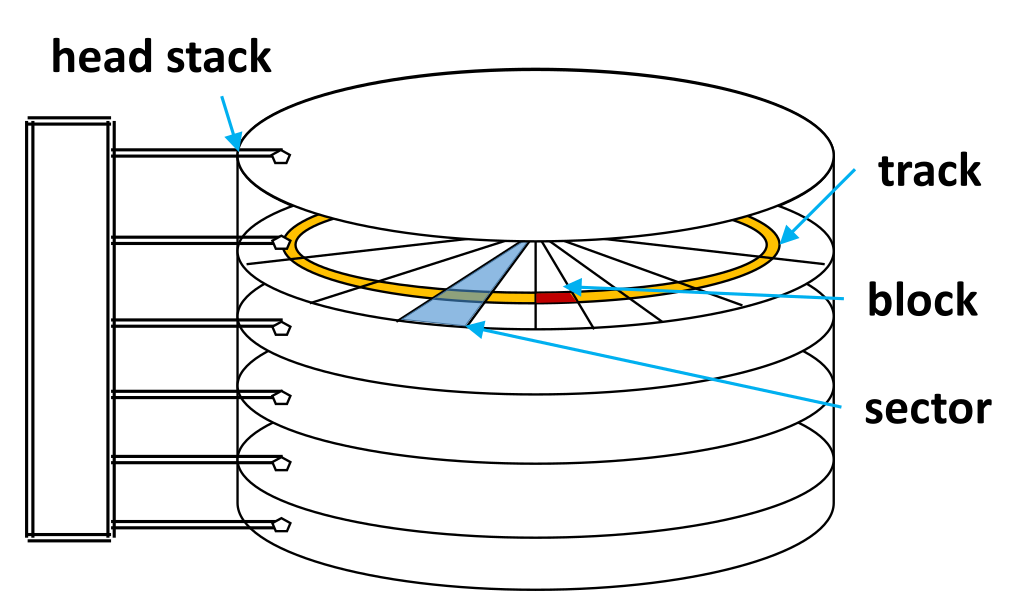
\includegraphics{hdd-structure.png}
  }
  \caption{Structure of a mechanical hard drive}
  \label{figure:hdd-structure}
  \bigskip
\end{figure}

\subparagraph*{Access Time}
The access time of the secondary memory can be measured as the sum of:
\begin{itemize}
  \item seek time \(8-12 \, ms\), head positioning time on the correct track
  \item latency time \(2-8 \, ms\), disc rotation on the correct sector
  \item transfer time \(0.1-1 \, ms\), data transfer from the disk to the buffer
\end{itemize}

The cost of access to secondary memory is about \(4\) orders of magnitude (\(10^4\)) higher than the one of access to main memory.
In I/O bound applications, the cost exclusively depends on the number of accesses to secondary memory.

The cost of a query is closely related to the number of numbers that are read (moved) from secondary memory.

\subparagraph*{\dbms and file systems}
The File System (FS) is the layer of the operating system that manages the secondary memory:
\dbms make limited use of FS functionalities (such as creating or deleting files, reading or writing blocks, etc.), since they manage directly the file organization, both in terms of the distribution of data within the blocks and with respect to the internal structures of the blocks.
Furthermore, a \dbms may also control the physical allocation of blocks onto the disk, to optimize the access time or increase the reliability.

\subsection{Blocks and tuples}

The files can be split into their physical and logical components:

\begin{itemize}
  \item \textbf{blocks}: the physical components
  \item \textbf{tuples}: the logical components
\end{itemize}

While the size of a block is typically fixed, depending on the file system and on how the disk is formatted, the size of a tuple depends on the database design and is typically variable within a file.

\subparagraph*{Organization of tuples in blocks}

A block for sequential and hash-based methods is divided in:

\begin{itemize}
  \item block header and trailer with control information used by the File System
  \item page header and trailer with control information about the access method
  \item a page dictionary containing pointers to each elementary item of useful data contained in the page
  \item a useful part containing the data
        \begin{itemize}
          \item normally, page dictionaries and useful data grow as a stack in opposite directions
        \end{itemize}
  \item a checksum to verify the integrity of the block
\end{itemize}

An illustration of a block is shown in Figure~\ref{fig:block-structure}.

\begin{figure}[htbp]
  \centering
  \bigskip
  \tikzfig{figure-14.tikz}
  \caption{Structure of a block}
  \label{fig:block-structure}
  \bigskip
\end{figure}

\bigskip
The block factor B represents the number of tuples within a block.
It's fundamental to estimate the cost of queries:

\begin{itemize}
  \item The average size of a record \textit{(or tuple)} is called \textbf{SR}
  \item The average size of a block is called \textbf{SB}
\end{itemize}

Then the block factor is:
\[ B = \lfloor \frac{\text{SB}}{\text{SR}} \rfloor \]
The rest of the space can be:

\begin{itemize}
  \item used if the records are spanned between block
  \item not used, if the records are unspanned
\end{itemize}

\subparagraph*{Buffer Operations}

Operations are performed in the main memory and affect the pages: in the cost model, it's always assumed that all the pages have equal size and are organized in blocks.

Operations are:

\begin{itemize}
  \item insertion an update of a tuple
        \begin{itemize}
          \item may require a reorganization of the page or the usage of a new page
          \item an update to a file may require a reorganization of the page
        \end{itemize}
  \item deletion of a tuple
        \begin{itemize}
          \item often carried out by marking the tuple as invalid and triggering later a reorganization of the page
        \end{itemize}
  \item access to a field of a tuple
        \begin{itemize}
          \item identified by a pointer to the beginning of the tuple and the length of the field itself
        \end{itemize}
\end{itemize}

\subsection{Indexes}

Indexes are data structures that help efficiently retrieve tuples according to certain criteria, called \textbf{search key} (or \textit{SK}).
They contain records in the form \(\langle \text{search key}, \text{pointer to block} \rangle\); index entries are sorted with regard to the search key.

It's important to highlight the difference between \textbf{primary key} and \textbf{search key}:
the former is the key used to uniquely identify a tuple, while the latter is the key used to retrieve tuples according to certain criteria.
Furthermore, the search key defines a \textbf{search domain}: each tuple is associated with one or more pointers; each of them may not be unique.

A comparison of the two entities is shown in Table~\ref{tab:primary-key-search-key}.

\begin{table}[htbp]
  \centering
  \bigskip
  \begin{tblr}{colspec={c|c}, row{1}={font=\itshape}}
    primary key                & search key                   \\
    \hline
    does not imply access path & defines a common access path \\
    defines a constraint       & defines a common access path \\
    unique                     & not necessarily unique       \\
    implemented by an index    &                              \\
  \end{tblr}
  \caption{Comparison between primary key and search key}
  \label{tab:primary-key-search-key}
  \bigskip
\end{table}

Indexes are smaller than primary data structures, and they can be loaded in a file in the main memory;
they support point queries, range queries, and sorted scans efficiently.
However, adding indexes to tables means that the \dbms has to update each index after an insert, update, or delete operation:
this operation may be costly and may slow down the \dbms.

\bigskip
Indexes can be categorized into \textbf{sparse} and \textbf{dense}:
while the former associate a search key to a single tuple, the latter associate a search key to a block of tuples.

\subparagraph*{Sparse indexes}
\begin{itemize}
  \item an entry index is associated with \textbf{every} search-key value in the file
  \item high performances: in order to access a tuple, the index is accessed first, then the block is accessed
  \item can be used on entry-sequenced primary structures
\end{itemize}

\subparagraph*{Dense indexes}
\begin{itemize}
  \item an entry index is associated only with \textbf{some} search-key values in the file
  \item requires less space, but it's generally slower in locating the tuple
  \item requires sequentially ordered primary structures
        \begin{itemize}[label=\(\rightarrow\)]
          \item the search key corresponds to the ordering key of the tuple
        \end{itemize}
  \item low performances: in order to access a tuple, it's necessary to scan each block until the search key is found; then the block must be scanned to locate the tuple itself
  \item Good tradeoff between memory and performance as only one index entry is necessary for each block in the file
\end{itemize}

\subsubsection{Indexing techniques}

The index can be further classified according to the indexing used, creating the following indexes: \textbf{primary}, \textbf{secondary}, and \textbf{clustering}.

\subparagraph*{Primary index}
A primary index is defined on sequentially ordered structures.
The search key (SK) is unique and coincides with the attribute according to which the structure is ordered:
\begin{align*}
  \text{search key} \  & = \ \text{ordering key} \\
  \text{SK} \          & = \ \text{OK}
\end{align*}

\begin{itemize}
  \item Only one primary index can be defined for each table
        \begin{itemize}
          \item usually the primary index corresponds to the primary key of the table
        \end{itemize}
  \item The index can be either \textbf{sparse} or \textbf{dense}
\end{itemize}

\subparagraph*{Secondary index}
A secondary index specifies an order different from the sequential order of the file:
\begin{align*}
  \text{search key} \  & \neq \ \text{ordering key} \\
  \text{SK} \          & \neq \ \text{OK}
\end{align*}

\begin{itemize}
  \item Multiple secondary indexes can be defined for the same table on multiple search keys
  \item It is always \textbf{dense} because tuples with contiguous values of the key can be distributed in different blocks
\end{itemize}

\subparagraph*{Clustering index}
A clustering index is a generalization of the primary index in which the ordering key (equal to the search key) can not be unique.

\begin{itemize}
  \item The pointer of key \texttt{x} refers to the block containing the first tuple with key \texttt{x}
  \item The index can be either \textbf{sparse} or \textbf{dense}, but it is usually \textbf{sparse}
\end{itemize}

\subsection{Physical Access Structures}

Each \dbms has a distinctive and limited set of access methods and software modules that provide data access and manipulation (\texttt{STORE} and \texttt{RETRIEVE}) primitives for each physical data structure.

Access methods have their own data structures to organize data:

\begin{itemize}
  \item Each table is stored in exactly one primal physical data structure
  \item Each table may have one or more optional secondary access structures
\end{itemize}

\bigskip
Structures are divided in two \textbf{categories}:

\begin{itemize}
  \item \textbf{Primary}: contains  all the tuples of a table; its main purpose is store the table content
  \item \textbf{Secondary}: used to index primary structures, and only contains the values of some fields, interleaved with pointers to the block of the primary structure; its main purpose is to speed up the search for specific tuples, according to some criteria
\end{itemize}

To access each type of structure, the \dbms uses a different set of access methods:

\begin{itemize}
  \item \textbf{Sequential} access methods
  \item \textbf{Hash-based} access methods
  \item \textbf{Tree-based} access methods
\end{itemize}

Not all types of structures are equally suited for implementing the primary or secondary access methods, as shown in Table~\ref{tab:access-structures}.

\begin{table}
  \centering
  \bigskip
  \begin{tblr}{colspec={r|l|l}, row{1}={font=\itshape}, column{1}={font=\bfseries}}
               & primary                     & secondary             \\
    \hline
    sequential & \colorcmark (typical)       & \colorxmark           \\
    hash-based & \colorcmark (in some \dbms) & \colorcmark           \\
    tree-based & \colorxmark (obsolete)      & \colorcmark (typical)
  \end{tblr}
  \caption{Access structures}
  \label{tab:access-structures}
  \bigskip
\end{table}

\subsubsection{Sequential structures}
Sequential structures arrange tuples in a sequence in the secondary memory;
blocks can be contiguous on disk or sparse.

Two types of sequential structures are:

\begin{itemize}
  \item entry-sequenced organization: the sequence of tuples is dictated by their entry order
  \item sequentially-ordered organization: the sequence of tuples is dictated by the value of one or more keys
\end{itemize}

\subparagraph*{Entry-sequenced organization} Entry-sequenced organization \textit{(also called heap)} is the simplest and most common type of sequential organization.

\begin{itemize}
  \item Efficient for:
        \begin{itemize}[label=\cmarkthin]
          \item insertion, which does not require shifting
          \item space occupancy, as it uses all the blocks available for data and all the space within a block
          \item sequential reading and writing, especially if the blocks are contiguous
          \item query like \texttt{SELECT * FROM table}
        \end{itemize}
  \item Inefficient for:
        \begin{itemize}[label=\xmarkthin]
          \item searching specific data units, as it may require scanning the whole structure
                \begin{itemize}[label=\(\rightarrow\)]
                  \item this issue can be solved via indexes
                \end{itemize}
          \item updates that increase the size of a tuple, as it may require shifting and writing on another block
                \begin{itemize}[label=\(\rightarrow\)]
                  \item this issue can be solved by deleting old versions of the tuple and inserting new ones
                \end{itemize}
          \item query like \texttt{SELECT * FROM table WHERE ...}
        \end{itemize}
\end{itemize}

\subparagraph*{Sequentially-ordered sequential structure}
Tuples are sorted according to the value of a key field.

\begin{itemize}
  \item Efficient for:
        \begin{itemize}[label=\cmarkthin]
          \item range queries that retrieve tuples having the key in an interval
          \item \texttt{order by} and \texttt{group by} queries exploiting the key
        \end{itemize}
  \item Inefficient for:
        \begin{itemize}[label=\xmarkthin]
          \item reordering tuples within a block, if there is even enough space
        \end{itemize}
\end{itemize}

In order to avoid the global reordering problem, the following techniques can be used:

\begin{itemize}
  \item Differential files and periodic merging
  \item Local reordering operation within a block
  \item Creation of an overflow file that contains tuples that do not fit in the current block
\end{itemize}

\paragraph{Comparison of sequential structures}

Table~\ref{tab:sequential-structures} shows the main differences between the main structures.

In real-world applications, the entry-sequenced organization is the most common solution only if paired with secondary access structures.

\begin{table}[htbp]
  \centering
  \bigskip
  \begin{tblr}{colspec={r|c|c}, row{1}={font=\itshape}, column{1}={font=\ttfamily}}
               & entry-sequenced   & sequentially-ordered \\
    \hline
    tuple size & fixed or variable & fixed or variable    \\
    INSERT     & \colorcmark       & \colorxmark          \\
    UPDATE     & \colorcmark       & \colorxmark          \\
    DELETE     & \colorxmark       & \colorxmark          \\
    {SELECT * FROM T                                      \\ WHERE ...} & \colorxmark & \colorcmark \\
  \end{tblr}
  \caption{Comparison of sequential structures}
  \label{tab:sequential-structures}
  \bigskip
\end{table}

\subsubsection{Hash-based structures}

Hash-based structures provide efficient associative access to data, based on the value of a key field.

A hash-based structure has \(N_B\) buckets, with \(N_B \ll \# \text{of data items}\):
a bucket is a unit of storage, typically of the size of \(1\) block;
often they are stored adjacently in the file.
A hash function maps the key field to a value between \(0\) and \(N_B -1\);
this value is interpreted as the index of a bucket in the hash structure (via a hash table).

\begin{itemize}
  \item Efficient for:
        \begin{itemize}[label=\cmarkthin]
          \item tables with small size and almost static content
          \item queries with equality predicates on the key field (point queries)
        \end{itemize}
  \item Inefficient for:
        \begin{itemize}[label=\xmarkthin]
          \item tables with large size and dynamic content
          \item queries with inequality predicates on the key field (range queries)
        \end{itemize}
\end{itemize}

\subparagraph*{Implementation}
The implementation consists of two parts.

\begin{enumerate}
  \item \textbf{folding}: transforms the key values to positive integers, uniformly distributed in a big range
  \item \textbf{hashing}: transforms the positive number into an index in range \(\left[ 0, N_B - 1 \right]\), to be used as the index of a bucket
\end{enumerate}

\subparagraph*{Collision}
When two or more keys are mapped to the same bucket, a \textbf{collision} occurs;
when the number of tuples in a block is greater than the number of buckets, collisions are inevitable;

Techinques to solve collisions:

\begin{itemize}
  \item \textbf{Closed hashing} \textit{(open addressing)}, where the collision is resolved by probing the next bucket
        \begin{itemize}[label=\(\rightarrow\)]
          \item a simple technique is linear probing, where the following buckets are tried in sequence wrapping around the end of the hash table
        \end{itemize}
  \item \textbf{Open hashing} \textit{(separate chaining)}, where the collision is resolved by storing the tuple in a linked list
        \begin{itemize}[label=\(\rightarrow\)]
          \item a new bucket is allocated for the same hash result linked to the previous one
        \end{itemize}
\end{itemize}

\subparagraph*{Overflow chains}
The average length of the overflow chain is a function of:

\begin{itemize}
  \item the load factor \(\alpha = \dfrac{T}{B \times N_B}\), representing the average occupancy of a block
  \item the block factor \(\beta = \frac{B}{\# \ \text{of items}} = \dfrac{1}{\alpha}\), representing the average number of items per block
\end{itemize}

Remember that:

\begin{itemize}
  \item \(T\) is the number of tuples
  \item \(N_B\) is the number of buckets
  \item \(B\) is the number of tuples within a block
\end{itemize}

\paragraph{Hash-based indexes}

Hash-based structures can be used for secondary indexes:
they are shaped and managed exactly like a hash-based primary structure, but instead of the tuples, the buckets contain key values and pointers.

In a huge database it would be very inefficient to search all the index values to reach the desired data:
a good performance equality query predicates on the key field.

This technique is then inefficient for access based on interval predicates or on the value of non search-key attributes.
% TODO write something more

\subsubsection{Tree-based structures}

The tree-based structures are the most frequently used in relational \dbms for secondary index structures;
for instance, \sql structures are implemented this way.
They support associative access based on the value of a key search field.

A commonly used tree-based structure is the \textbf{B-tree}.

\subparagraph*{B-trees}
Balanced trees (or B-trees) are a generalization of binary search trees;
the length of all the possible paths from the root node to the leaves is the same.
This constraint improves the performance of the database.

There are two types of b trees:

\begin{enumerate}
  \item \textbf{B trees}: the key values are stored in \textbf{leaf nodes and internal nodes}
  \item \textbf{B+ trees}: the key values are stored in \textbf{leaf nodes} only
\end{enumerate}

\paragraph{B+ trees}

The \textbf{B+ tree} represents an evolution from the B-tree.
Each node is stored in a block, and the key values are stored in the leaf nodes only;
since the majority of the nodes are leaf nodes, the B+ tree is more efficient than the B-tree.

The fan-out depends on the size of the block, the size of the key and the size of the pointer.

\subparagraph*{Structure of an internal node}
The structure of an internal node is shown in Figure~\ref{subfig:b-tree-internal-node}.
Each node contains \(F\) keys, sorted lexicographically, and \(F + 1\) pointers to the child nodes.
Each key \(K_j, \ 1 \leq j \leq F\) is followed by a pointer \(P_j\), while \(K_1\) is preceded by a pointer \(P_0\).
Each pointer addresses a sub-tree:

\begin{itemize}
  \item \(P_0\) points to the subtree containing all the keys less than \(K_1\)
  \item \(P_F\) points to the subtree containing all the keys greater or equal to \(K_F\)
  \item each intermediate pointer addresses a sub-tree that contains all the information about the keys \(K\) included in the interval \(K_j \leq K < K_{j + 1}\)
\end{itemize}

The value of \(F\) depends on the size of the page and on the amount of space occupied by the key values and the pointers.

\subparagraph*{Structure of a leaf node}
The structure of a leaf node is similar to the one of an internal node, but it contains only pointers to the data tuples or the data tuples themselves;
the nodes can be structured in two ways:

\begin{enumerate}
  \item the leaf node contains the entire tuple
        \begin{itemize}
          \item the data structure is called \textbf{key-sequenced}
          \item the position of a tuple is determined by the value of its key
          \item it's simple to insert or change a tuple
        \end{itemize}
  \item the leaf node contains pointers to the blocks of the database that contain tuples with the same key value
        \begin{itemize}
          \item the data structure is called \textbf{indirect}
          \item the tuples can be anywhere in the file, allowing the access of a tuple allocated via any other primary mechanism
          \item the structure of such a leaf node is shown in Figure~\ref{subfig:b-tree-leaf-node}
        \end{itemize}
\end{enumerate}

\begin{figure}[htbp]
  \centering
  \bigskip
  \begin{subfigure}{0.99\textwidth}
    \centering
    \bigskip
    \tikzfig{figure-15.tikz}
    \caption{Internal node}
    \label{subfig:b-tree-internal-node}
    \bigskip
  \end{subfigure}
  \bigskip
  \begin{subfigure}{0.99\textwidth}
    \centering
    \bigskip
    \tikzfig{figure-16.tikz}
    \caption{Leaf node}
    \label{subfig:b-tree-leaf-node}
    \bigskip
  \end{subfigure}
  \caption{Structure of the nodes of a B+ tree}
  \label{fig:b-tree-structure}
\end{figure}

\paragraph{Search Mechanism}

The search mechanism consists of the following pointers starting from the root.
At each intermediate node:

\begin{itemize}
  \item if \(V < K_1\), follow the pointer \(P_0\)
  \item If \(V \geq K_F\), follow the pointer \(P_F\)
  \item otherwise, follow the pointer \(P_j\) such that \(K_j \leq V < K_{j + 1}\)
\end{itemize}

The search continues until a leaf node is found:

\begin{itemize}
  \item in case of a key-sequenced leaf node, the search is completed as the tuple is found
  \item in case of an indirect leaf node, it's necessary to access the memory block pointed by the pointer \(P_j, \ 0 \leq j \leq F\)
\end{itemize}

\subsection{Structures and Indexes}

A comparison of indexing methods related to the data structures is shown in Table~\ref{tab:indexing-techniques}.

\begin{table}[htbp]
  \centering
  \bigskip
  \begin{tblr}{colspec={c|c|c|c|c}, row{1}={font=\itshape}, cells={valign=m}}
    type of index & type of structure & search key & ordering & allowed number of indexes \\
    \hline
    primary       & {sequential                                                           \\ with SK \(=\) OK} & unique & dense or sparse & one per table \\
    secondary     & {sequential                                                           \\ with SK \(\neq\) OK} & unique or not & dense & many per table \\
    clustering    & {sequential                                                           \\ with SK \(=\) OK} & not unique & normally sparse & one per table \\
  \end{tblr}
  \caption{Comparison of the three indexing techniques}
  \label{tab:indexing-techniques}
  \bigskip
\end{table}

\clearpage

\section{Tricky Exercises and how to slay them}

\subsection{Concurrency Control}

\subsubsection{Schedule classification}

Due to the presence of blind writes, the \CG of a schedule is cyclic;
as such, it's not in \CSR.
By swapping two of the nodes in the \CG, it may be possible to obtain a schedule that is in \VSR;
if it's not possible, then the schedule is not in \VSR either.

In some schedules, the blind writes may appear multiple times involving the same transactions with different objects in different orders;
in such cases the schedule is not in \CSR \textit{(and thus not in \VSR)}.

\paragraph{\TPL}

It's necessary to impose temporal constraints on the lock and unlock requests, based on two principles:

\begin{itemize}
  \item \textbf{same resource} \(R\) - each lock can be acquired if \(R\) is free
        \[ {U^r_i}^R < {L^w_j}^R \quad {U^w_i}^R < {L^r_j}^R \quad {U^w_i}^R < {L^w_j}^R \qquad i \neq j \]
  \item \textbf{same transaction} \(i\) - all releases must follow all acquisitions
        \[{L^{r/w}_i}^{R_n} < {L^{r/w}_i}^{R_m} \qquad n \neq m \]
\end{itemize}

The instants in which the actions take place, in to write inequalities.
This approach is needed because the non-strict \TPL does not allow showing when a transaction has released a lock.

\subsubsection{Update lock}

A common notation to avoid ambiguity between Unlock and Update is to use the notation \(\texttt{SL}_i(x)\) for a \texttt{SL} request on resource \(x\) by transaction \(T_i\) and \(\texttt{rel}(\texttt{SL}_i(x))\) for the corresponding release.

In order to avoid deadlocks due to interleaved lock upgrades, any upgrade \(\texttt{SL} \rightarrow \texttt{XL}\) is not allowed;
the transaction needs to acquire a \texttt{UL} lock first and then upgrade it to a \texttt{XL} lock.

\end{document}